\section{Construção {\it naive} $O(N^2)$ da {\it trie}}

\begin{frame}[fragile]{Construção {\it naive} da {\it trie}}

    \begin{itemize}
        \item Seja $s$ uma string de tamanho $N$
        \pause

        \item Cada nó da {\it trie} de $s$ pode ter até $|A|$ filhos, onde $A$ é o alfabeto
        \pause

        \item Assim, cada nó pode ser implementado como um vetor de pares ou como um mapa,
            onde o par $(c, n)$, indicando que há uma aresta de rótulo $c$ que aponta para o
            nó $n$
        \pause

        \item A raiz da árvore será o nó identificado por $n = 0$
        \pause

        \item Para cada caractere $c$ do sufixo $s[i..N]$, e iniciando na raiz,
            verifica-se se existe a aresta $(c, n)$
        \pause

        \item Em caso, afirmativo, segue-se esta aresta e se processa o caractere que sucede $c$
        \pause

        \item Caso não exista, cria-se um novo nó $m$, adiciona-se ao nó atual a aresta
            $(c, m)$, e segue o processamento para $m$ e para o próximo caractere
        \pause
    
        \item Esta construção tem complexidade $O(N^2)$
        \pause

        \item A memória necessária também é $O(N^2)$
    \end{itemize}

\end{frame}

\begin{frame}[fragile]{Implementação {\it naive} da {\it trie}}
    \inputsnippet{cpp}{1}{20}{codes/trie_naive.cpp}
\end{frame}

\begin{frame}[fragile]{Implementação {\it naive} da {\it trie}}
    \inputsnippet{cpp}{22}{35}{codes/trie_naive.cpp}
\end{frame}

\begin{frame}[fragile]{Busca de substring em um {\it trie}}

    \begin{itemize}
        \item A \textit{trie} da string $s$ pode ser utilizada para identificar se uma string 
            $p$ é ou não substring de $s$
        \pause

        \item O algoritmo é semelhante à busca em uma árvore binária, e tem complexidade $O(m)$, onde $m = |p|$
        \pause

        \item Por exemplo, se $s = $ \code{cpp}{"BANANA"} e $p = $ \code{cpp}{"NAN"}, partindo da 
            raiz, tem-se \code{cpp}{"N"} na aresta à direita, \code{cpp}{"A"} na única 
            aresta e \code{cpp}{"N"} na aresta seguinte: logo $p$ é substring de $s$
        \pause

        \item Como o nó de chegada é branco, $p$ não é sufixo de $s$
        \pause

        \item Para $p =$ \code{cpp}{"NAS"}, o último caractere (\code{cpp}{"S"}) não seria 
            encontrado
        \pause

        \item O mesmo vale para $p = $ \code{cpp}{"MAS"}, porém a falha acontece logo no primeiro 
            caractere
        \pause

        \item Para $p = $ \code{cpp}{"NANAN"} a busca se encerraria ao atingir um nó nulo

    \end{itemize}

\end{frame}

\begin{frame}[fragile]{Implementação da busca em $O(m)$ em uma {\it trie}}
    \inputsnippet{cpp}{66}{81}{codes/trie_naive.cpp}
\end{frame}

\begin{frame}[fragile]{{\it Trie} com marcadores}

    \begin{itemize}
        \item A construção proposta para a \textit{trie} permite ao algoritmo de busca descrito 
            apenas determinar se a substring $p$ ocorre ou não em $s$
        \pause

        \item Se for preciso determinar a posição (ou posições) desta ocorrência, é preciso 
            modificar a construção da \textit{trie}, de modo que seja possível discriminar os nós 
                essenciais dos demais
        \pause

        \item Uma maneira de fazê-lo é adicionar um caractere terminador (em geral, o caractere
            `\texttt{\#}'), que não pertença a string original
        \pause

        \item A este caractere estará associado o índice $i$ da string tal que o sufixo terminado 
            no marcador é igual a $S[i..N]$
        \pause

        \item Importante notar que o segundo elemento do par terá dois significados distintos: ou
            será um ponteiro para o próximo nó, ou o índice do sufixo caso o rótulo da aresta
            seja o terminador
        \pause

        \item É preciso atentar a esta diferença na implementação das rotinas de construção e
            busca
    \end{itemize}

\end{frame}

\begin{frame}[fragile]{Visualização da {\it trie} da palavra {\tt `BANANA'} com terminador {\tt \#}}

    \begin{figure}
        \centering

        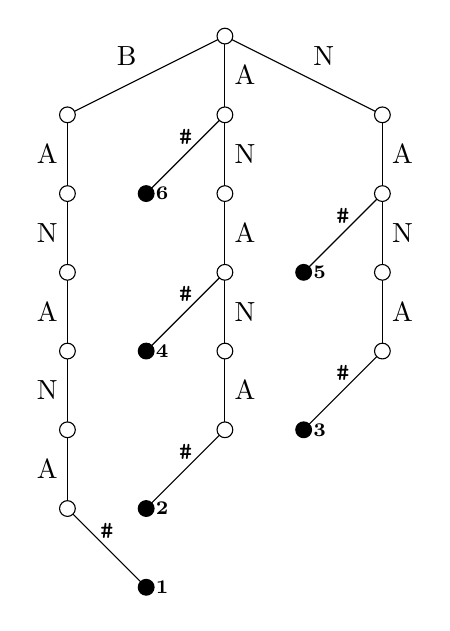
\begin{tikzpicture}
            \coordinate (A) at (4, 7);
            \coordinate (B1) at (2, 6);
            \coordinate (B2) at (4, 6);
            \coordinate (B3) at (6, 6);
            \coordinate (B4) at (3, 5);
            \coordinate (C1) at (2, 5);
            \coordinate (C2) at (4, 5);
            \coordinate (C3) at (6, 5);
            \coordinate (C4) at (5, 4);
            \coordinate (D1) at (2, 4);
            \coordinate (D2) at (4, 4);
            \coordinate (D3) at (6, 4);
            \coordinate (D4) at (3, 3);
            \coordinate (E1) at (2, 3);
            \coordinate (E2) at (4, 3);
            \coordinate (E3) at (6, 3);
            \coordinate (E4) at (5, 2);
            \coordinate (F1) at (2, 2);
            \coordinate (F2) at (4, 2);
            \coordinate (F3) at (3, 1);
            \coordinate (G1) at (2, 1);
            \coordinate (G2) at (3, 0);

            \draw (A) -- node[anchor=south east] { B } (B1);
            \draw (A) -- node[anchor=west] { A } (B2);
            \draw (A) -- node[anchor=south west] { N } (B3);
            \draw (B1) -- node[anchor=east] { A } (C1);
            \draw (B2) -- node[anchor=west] { N } (C2);
            \draw (B3) -- node[anchor=west] { A } (C3);
            \draw (B2) -- node[anchor=south] { \tt \small \# } (B4);
            \draw (C1) -- node[anchor=east] { N } (D1);
            \draw (C2) -- node[anchor=west] { A } (D2);
            \draw (C3) -- node[anchor=west] { N } (D3);
            \draw (C3) -- node[anchor=south] { \tt \small \# } (C4);
            \draw (D1) -- node[anchor=east] { A } (E1);
            \draw (D2) -- node[anchor=west] { N } (E2);
            \draw (D3) -- node[anchor=west] { A } (E3);
            \draw (D2) -- node[anchor=south] { \tt \small \# } (D4);
            \draw (E1) -- node[anchor=east] { N } (F1);
            \draw (E2) -- node[anchor=west] { A } (F2);
            \draw (E3) -- node[anchor=south] { \tt \small \# } (E4);
            \draw (F1) -- node[anchor=east] { A } (G1);
            \draw (F2) -- node[anchor=south] { \tt \small \# } (F3);
            \draw (G1) -- node[anchor=south] { \tt \small \# } (G2);

            \draw[fill=white] (A) circle [radius=.1];

            \draw[fill=white] (B1) circle [radius=.1];
            \draw[fill=white] (B2) circle [radius=.1];
            \draw[fill=black] (B4) circle [radius=.1] node[anchor=west] { \scriptsize \bf 6 };
            \draw[fill=white] (B3) circle [radius=.1];
            \draw[fill=white] (C1) circle [radius=.1];
            \draw[fill=white] (C2) circle [radius=.1];
            \draw[fill=white] (C3) circle [radius=.1];
            \draw[fill=black] (C4) circle [radius=.1] node[anchor=west] { \scriptsize \bf 5 };
            \draw[fill=white] (D1) circle [radius=.1];
            \draw[fill=white] (D2) circle [radius=.1];
            \draw[fill=white] (D3) circle [radius=.1];
            \draw[fill=black] (D4) circle [radius=.1] node[anchor=west] { \scriptsize \bf 4 };
            \draw[fill=white] (E1) circle [radius=.1];
            \draw[fill=white] (E2) circle [radius=.1];
            \draw[fill=white] (E3) circle [radius=.1];
            \draw[fill=black] (E4) circle [radius=.1] node[anchor=west] { \scriptsize \bf 3 };
            \draw[fill=white] (F1) circle [radius=.1];
            \draw[fill=white] (F2) circle [radius=.1];
            \draw[fill=black] (F3) circle [radius=.1] node[anchor=west] { \scriptsize \bf 2 };
            \draw[fill=white] (G1) circle [radius=.1];
            \draw[fill=black] (G2) circle [radius=.1] node[anchor=west] { \scriptsize \bf 1 };


        \end{tikzpicture}
    \end{figure}

\end{frame}

\begin{frame}[fragile]{Construção da {\it trie} com marcador}
    \inputsnippet{cpp}{83}{102}{codes/trie_naive.cpp}
\end{frame}

\begin{frame}[fragile]{Construção da {\it trie} com marcador}
    \inputsnippet{cpp}{104}{117}{codes/trie_naive.cpp}
\end{frame}

\begin{frame}[fragile]{Identificação das ocorrências de uma substring em uma {\it trie} com marcadores}
    \inputsnippet{cpp}{119}{136}{codes/trie_naive.cpp}
\end{frame}

\begin{frame}[fragile]{Identificação das ocorrências de uma substring em uma {\it trie} com marcadores}
    \inputsnippet{cpp}{137}{152}{codes/trie_naive.cpp}
\end{frame}

\begin{frame}[fragile]{Número de substrings distintas}

    \begin{itemize}
        \item Outra informação que pode ser obtida a partir da \textit{trie} é o número de 
            substring distintas de $s$
        \pause

        \item Se $s$ tem $n$ caracteres, ela terá $n(n + 1)/2$ substrings não vazias, não 
            necessariamente distintas
        \pause

        \item Estas substrings correspondem a todos os pares de índices $(i, j)$, com 
            $i \leq j$, onde $i, j = 1, 2, \ldots, n$
        \pause

        \item Em uma \textit{trie}, qualquer nó, exceto a raiz, representa uma substring 
            distinta, formada pela concatenação dos rótulos do caminho da raiz até o nó em
            questão
    \end{itemize}

\end{frame}

\begin{frame}[fragile]{Contagem de substrings distintas em uma {\it trie}}
    \inputsnippet{cpp}{154}{173}{codes/trie_naive.cpp}
\end{frame}

\begin{frame}[fragile]{Considerações sobre a construção {\it naive} da {\it trie}}

    \begin{itemize}
        \item Embora as buscas apresentadas satisfaçam o terceiro critério para uma boa árvore de 
            sufixo, os outros dois critérios não são satisfeitos
        \pause

        \item Se a string $s$ inicial tem $N$ caracteres, a construção e o espaço em memória são 
            $O(N^2)$.
        \pause

        \item É possível melhorar a complexidade da construção da {\it trie}, por meio de um
            algoritmo \textit{online}
        \pause

        \item O espaço em memória, contudo, permanecerá $O(N^2)$, por conta da representação de
            cada caractere por meio de uma aresta
        \pause

        \item Assim, a redução de memória só é possível por meio de uma mudança na representação
            dos caracteres e dos sufixos, o que leva a uma outra estrutura, a \textit{suffix trie}
    \end{itemize}

\end{frame}
